\section{Exponencial}\label{cons:exp}

\subsection{Motivación: (De)construyendo el exponencial}

Nos interesa comenzar esta sección evocando una problemática simple de la combinatoria de la matemática discreta y preguntarnos: ¿cuántas funciones existen entre dos conjuntos cualesquiera $A$ y $B$?

En la figura \ref{fig:funciones} vemos un ejemplo muy sencillo de dos conjuntos $A$ y $B$ y tres funciones posibles de un conjunto al otro. Se muestran las posibilidades dada una elección determinada de asignación al elemento $a_1$. Tenemos tantas opciones de mapeo para $a_2$ como elementos hay en $B$. La misma cantidad de alternativas existen para asignar a $a_1$.


\begin{figure}[H] 
\begin{center}
  \xymatrixcolsep{0.5pc} \xymatrixrowsep{2pc}
  \centerline{
  \xymatrix{ 
      A \ = & \{ a_{1}, \ar@{|->}[d]  & a_{2} \ar@{|->}[dl]   \} \\
      B \ = & \{ b_{1}, & b_{2}, & b_{3} \} }
  \quad
  \xymatrix{ 
       \{ a_{1},  \ar@{|->}[d] & a_{2}, \ar@{|->}[d] \} \\
       \{ b_{1}, & b_{2} , & b_{3}\} }
    \quad
  \xymatrix{ 
       \{ a_{1},  \ar@{|->}[d] & a_{2}, \ar@{|->}[dr]  \} \\
       \{ b_{1}, & b_{2}, & b_{3} \} }}
  %% \vspace{2ex}
  %% \centerline{
  %% \xymatrix{ 
  %%     \hspace{4ex}& \{ a_{1}, \ar[dr]  & a_{2} \ar[dl]   \} \\
  %%     \hspace{4ex}& \{ b_{1}, & b_{2}, & b_{3} \} }
  %% \quad
  %% \xymatrix{ 
  %%      \{ a_{1},  \ar[dr] & a_{2}, \ar[d] \} \\
  %%      \{ b_{1}, & b_{2} , & b_{3}\} }
  %%   \quad
  %% \xymatrix{ 
  %%      \{ a_{1},  \ar[dr] & a_{2}, \ar[dr]  \} \\
  %%      \{ b_{1}, & b_{2}, & b_{3} \} }}
  %% \vspace{2ex}
  %% \centerline{
  %% \xymatrix{ 
  %%     \hspace{4ex}& \{ a_{1}, \ar[drr]  & a_{2} \ar[dl]   \} \\
  %%     \hspace{4ex}& \{ b_{1}, & b_{2}, & b_{3} \} }
  %% \quad
  %% \xymatrix{ 
  %%      \{ a_{1},  \ar[drr] & a_{2}, \ar[d] \} \\
  %%      \{ b_{1}, & b_{2} , & b_{3}\} }
  %%   \quad
  %% \xymatrix{ 
  %%      \{ a_{1},  \ar[drr] & a_{2}, \ar[dr]  \} \\
  %%      \{ b_{1}, & b_{2}, & b_{3} \} }}
\label{fig:funciones}
\end{center}
\caption{Algunas funciones entre los conjuntos $A$ y $B$ }
\end{figure}

Observemos que si los conjuntos $A$ y $B$ tienen respectivamente $a$ y $b$ cantidad de elementos, tenemos, por cada elemento de $A$, $b$ opciones de mapeos; entonces existen $$\underbrace{b \times b \times  \cdots  b}_{a \text{ veces}} = b^{a}$$
funciones posibles. Por dicha razón, al conjunto de las funciones de $A$ hacia $B$ le asignamos el nombre de exponencial de $B$ a la $A$, y lo simbolizamos $B^{A}$.

En resumen, en la categoría $\Set$ de conjuntos y funciones, el objeto exponencial entre dos objetos $A$ y $B$ que denominamos $B^{A}$, es el conjunto de las funciones de $A$ en $B$. 

Para empezar a pensar en las funciones hacia cada conjunto exponencial, consideremos las funciones $f(\_,\_) : A \times B \to C$.
Al fijar un elemento $a \in A$ obtenemos una nueva función $f(a,\_) : B \to C$; en otras palabras, $f(a,\_) \in C^{B}$. Si hacemos nuevamente variar $a$ entre los elementos de $A$, obtenemos una nueva función que llamamos $\curry{f}$ tal que $$\curry{f} : A \to C^{B}$$ $$\curry{f} (a) = f(a, \_)$$
La función $\curry{f}$ suele llamarse {\it currificación} de $f$ en honor al matemático Haskell B. Curry. Definimos la currificación de una función $f$ como $\curry{f} (a)(b) = f(a,b)$. 

En resumidas cuentas, cualquier función que reciba dos argumentos puede ser currificada y obtener así una nueva función que recibe un solo argumento, retornando una función. Sin embargo, seguir el camino inverso también es posible; para toda función $g : A \to B \to C$ existe una única $\uncurry{g} : A \times B \to C$ tal que $g = \curry{\uncurry{g}}$. Podemos definirla como: $$\uncurry{g}(a,b) = g(a)(b)$$  

Es simple de probar que nos encontramos --para cada conjunto $C^B$-- frente a una serie de isomorfismos en $\Set$, uno por cada conjunto $A$. Si tenemos las funciones $f : A \times B\to C$ y $g : A\to C^{B}$ entonces vemos que se cumple que las dos posibles composiciones de las funciones $\curry{\_}$ y $\uncurry{\_}$ dan como resultado las respectivas identidades.

$\uncurry{\curry{f}}(a,b) = \curry{f}(a)(b) = f(a,b) $

$\curry{\uncurry{g}}(a)(b) = \uncurry{g}(a,b) = g(a)(b) $

\subsection{Definición y formalización}
Antes de continuar con la presentación categórica del objeto exponencial, veamos otro ejemplo de funtor que puede encontrarse en las categorías que cuentan con productos, y que nos será necesario para continuar con la exposición.

\begin{definition}\label{homprod}
Sea $\C$ una categoría con productos. Dados dos objetos $B$ y $C$ de $\C$, el funtor $Hom_{\C}(\_\times B, C)$ desde la categoría $\C^{op}$ hacia la categoría $\Set$ mapea:

  \begin{itemize}
  \item cada objeto $A$ de $\C$ hacia el conjunto de morfismos $Hom_{\C}(A\times B, C)$
  \item cada morfismo $\flecha{A'}{f}{A}$ hacia la función de post-composición $$\_ \circ (f \times \id{B}) : Hom_{\C}(A\times B,C) \to Hom_{\C}(A'\times B,C)$$
  \end{itemize}
  El siguiente diagrama muestra cómo transformamos un morfismo del primer conjunto en uno del segundo a partir de la post-composición, vemos cómo en la categoría $\C$, de componer un morfismo $\flecha{A\times B}{h}{C}$ con el morfismo $\flecha{A'\times B}{f \times \id{B}}{A\times B}$ obtenemos un morfismo de $A'\times B$ hacia $C$. 

\begin{center}
  \xymatrixcolsep{4pc} \xymatrixrowsep{4pc}
  \centerline{\xymatrix{
          A \times B \ar[r]^{h} & C  \\
      A ' \times B \ar[u]^{f \times \id{B}} \ar[ur]_{h \circ (f \times \id{B})} & } \qquad
}
\end{center}
  
\end{definition}

En el código asociado a la tesina se puede encontrar la formalización y prueba de este funtor,  
%% A continuación, la formalización y parte de la prueba de que dicha construcción es en efecto un funtor,
que habremos de llamar \AgdaFunction{HomProd}.
%% \begin{agdacode}{\it Formalización del funtor Hom$_{\C}(\_\times Y , Z)$} \label{code:homProd}
    
%% \ExecuteMetaData[latex/HomFunctor.tex]{homProd}  
%% \end{agdacode}

\begin{definition}\label{cat:exp}
  Sea $\C$ una categoría que cuenta con productos y sean $B$ y $C$ dos de sus objetos. Un objeto $C^{B}$ es el {\it exponencial} de $C$ a la $B$ siempre que exista un isomorfismo natural entre los funtores {\it Hom}$(\_\times B, C)$ y {\it Hom}$(\_, C^{B})$.

  Al igual que con el coproducto y el producto, diremos que una categoría {\it cuenta con exponenciales} cuando para todo par de objetos existe el exponencial entre ellos.
\end{definition}

Del análisis de la definición observamos que para que un objeto $C^B$ sea exponencial deberá existir una transformación natural $\curry{\_}: \mathit{Hom}(\_\times B, C) \Rightarrow \mathit{Hom}(\_,C^B)$ tal que para cada $A$, cada una de sus componentes $\curry{\_}_{A}$ es un isomorfismo. Llamaremos $\uncurry{\_}_{A}$ a cada una de las inversas. El siguiente diagrama lo expresa de una forma alternativa. La doble línea indica la presencia de un isomorfismo.

\begin{center}
\xymatrixcolsep{1pc}
  \begin{minipage}{0.1\linewidth}
    \begin{center}
      \centerline{ \xymatrix{ {} \\ {}  \ar@/^/^{\uncurry{\_}_{A}}[u] }}
    \end{center}
  \end{minipage}
  \begin{minipage}{0.2\linewidth}
    \vspace{2ex}
    \begin{center}
      \centerline{ \infer={A \to C^B}{A\times B\to C} }
    \end{center}
  \end{minipage}
  \begin{minipage}{0.1\linewidth}
    \begin{center}
      \centerline{ \xymatrix{ {} \ar@/^/^{\curry{\_}_{A}}[d] \\ {} }}
    \end{center}
  \end{minipage}
\end{center}

Para apreciar mejor las consecuencias de la ley de naturalidad que obtenemos de la transformación natural $\curry{\_}$, observemos el siguiente diagrama conmutativo. Para todo par de objetos $A$ y $A'$ y morfismo $f : A' \to A$ de la categoría $\C^{op}$, el siguiente diagrama deberá conmutar.

\begin{center}
  \xymatrixcolsep{4pc} \xymatrixrowsep{3pc}
  \centerline{\xymatrix{ 
      \mathit{Hom}(A\times B,C) \ar[r]^{\_\circ(f\times \id{B})} \ar@/_/[d]_{\curry{\_}_{A}} & \mathit{Hom}(A'\times B,C) \ar@/_/[d]_{\curry{\_}_{A'}}\\
      \mathit{Hom}(A,C^B) \ar[r]_{\_ \,\circ\, f} \ar@/_/[u]_{\uncurry{\_}_{A}}& \mathit{Hom}(A',C^B)  \ar@/_/[u]_{\uncurry{\_}_{A'}}
}}
\end{center}
Además de los isomorfismos ya mencionados, se deberá pedir que se cumpla la ley de naturalidad dada por: $$\curry{g \circ (f \times \id{B})}_{A'} \cong \curry{g}_{A} \circ f \qquad \mbox{ para todo } g : A\times B \to C$$

Finalmente formalizamos el hecho de que una categoría $\C$ cuente con exponenciales con la estructura presentada en el código \ref{code:hasExponentials}. El campo \AgdaField{Exp} construye el objeto exponencial a partir de otros dos cualesquiera. El elemento \AgdaField{floor} es la transformación natural entre los funtores mencionados anteriormente, siendo el campo \AgdaField{nat} la formalización de la ley de naturalidad. Finalmente, el campo \AgdaField{ceil} construye cada uno de los isomorfismos requeridos, y la garantía de serlo está dada por los elementos \AgdaField{iso$_1$} e \AgdaField{iso$_2$}. 

\begin{agdacode}{\it Formalización de categoría con exponenciales}\label{code:hasExponentials}
 
\ExecuteMetaData[latex/Cat.tex]{hasExponentials}
\end{agdacode}

\begin{remark} Teniendo formalizados el concepto de isomorfismo natural (código \ref{code:natiso}) y los funtores \AgdaFunction{Hom$_1$} y \AgdaFunction{HomProd} (código \ref{code:hom1} y definición \ref{homprod}), podríamos haber formalizado \AgdaRecord{HasExponentials} como un record que contuviera simplemente al constructor \AgdaField{Exp} y un isomorfismo natural entre los funtores mencionados. Para mayor claridad, evitamos en este caso la construcción de records anidados.   
\end{remark}

\subsection{Exponencial de Containers}
En esta sección veremos que la categoría $\Cont$ de containers cuenta con exponenciales~\cite{alti:2010} y expondremos su formalización.

Con el objetivo presentar el exponencial de containers de la forma más comprensible posible, lo introduciremos a partir del análisis de un ejemplo, para luego presentarlo de forma general.

\begin{example} {\it Currificando} \AgdaFunction{append} 

  Para comenzar, recordemos que tenemos como objetivo construir, dados dos containers $B$ y $C$, su container exponencial, al que llamaremos $C$ \AgdaFunction{$\hat{\ }$} $B$. Dicho container deberá satisfacer las reglas de la definición, esto es, deberá existir un isomorfismo natural entre los siguientes morfismos de containers:

  $$
 \infer={A\ \AgdaFunction{$\Rightarrow$}\ C\ \AgdaFunction{$\hat{\ }$}\ B}{\AgdaDatatype{Both}\ A\ B\ \AgdaFunction{$\Rightarrow$}\ C} 
$$

 El morfismo \AgdaFunction{append} es un caso particular de morfismo de la parte superior del isomorfismo, instanciando $A$, $B$ y $C$ con el container \AgdaFunction{cList}.

   \ExecuteMetaData[latex/Examples.tex]{appendt}

   Buscamos construir un morfismo \AgdaFunction{curryappend} de tipo \AgdaDatatype{cList $\Rightarrow$ cList $\hat{\ }$ cList} isomorfo a \AgdaFunction{append}, es decir, sin pérdida de información, manteniendo la posibilidad de reconstruir \AgdaFunction{append} a partir de \AgdaFunction{curryappend}. Para ello, recordemos (ver ejemplo \ref{example:append}, pág. \pageref{example:append}) que el morfismo de concatenación arma un container de lista de longitud igual a la suma de las longitudes de las listas argumento; por otro lado, reubica las posiciones según la función \AgdaFunction{splitFin}, como se puede apreciar en la figura \ref{fig:append2}, donde la reubicación se indica con flechas.

\begin{figure}[H]
\begin{minipage}{0.3\textwidth}
\begin{center}
  \xymatrixrowsep{4pc} 
  \centerline{\xymatrix{ 
      \hspace{1ex}\ar@{=>}@/_1pc/[d]_{\mbox{\AgdaFunction{append}}} \\
      \hspace{1ex}
}}
\end{center}
\end{minipage}
     \begin{minipage}{0.7\textwidth}
  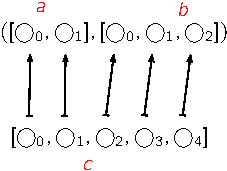
\includegraphics{img/append1.pdf}
     \end{minipage}
     \caption{Concatenación de containers de listas}
     \label{fig:append2}
\end{figure}

Podemos apreciar en la figura \ref{fig:curryappend} un panorama de general de comportamiento de la función \AgdaFunction{curryappend} y un esquema del objeto exponencial. Para referirnos con más exactitud a cada una de los containers de lista, los llamaremos \rojo{$a$}, \rojo{$b$} y \rojo{$c$}, de longitudes 2, 3 y 5 respectivamente. Así como en la figura \ref{fig:append2} representábamos al container producto $(\rojo{a},\rojo{b})$ entre paréntesis, ahora representamos al exponencial dentro del óvalo de la figura \ref{fig:curryappend}.

Las formas posibles del exponencial de dos listas incluirán no sólo una forma de construir la longitud de \rojo{$c$} a partir de las longitudes de las listas \rojo{$a$} y \rojo{$b$}, sino también la información de la reubicación de las posiciones de \rojo{$b$} en las posiciones de \rojo{$c$}. Más aún, se marcarán con un elemento distinguible \AgdaInductiveConstructor{tt} de tipo \AgdaDatatype{$\top$} a aquellas posiciones que se solían asignar a posiciones en \rojo{$a$}. Esto se ve representado en la figura \ref{fig:curryappend} con flechas rectas.

De esta forma, de las únicas posiciones que queda por determinar la procedencia son de aquellas marcadas con el valor \AgdaInductiveConstructor{tt}. Esas posiciones conformarán entonces el conjunto de posiciones del container exponencial. En el ejemplo de la figura \ref{fig:curryappend} encontramos dos de estas posiciones, representadas como aquellas de donde parten las flechas curvas.

\begin{figure}[H] 
\begin{minipage}{0.3\textwidth}
\begin{center}
  \xymatrixrowsep{5pc} 
  \centerline{\xymatrix{ 
      \hspace{1ex}\ar@{=>}@/_1pc/[d]_{\mbox{\AgdaFunction{curryappend}}} \\
      \hspace{1ex}
}}
\end{center}
\vspace{13ex}
\end{minipage}
\begin{minipage}{0.7\textwidth}
  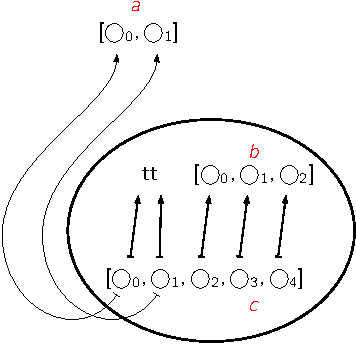
\includegraphics{img/curryappend1.pdf}
\end{minipage}
\caption{Currificación de la función de concatenación}
\label{fig:curryappend}
\end{figure}

Continuaremos con la presentación de este morfismo una vez presentada la construcción del exponencial de containers.
\end{example}


\begin{definition}\label{def:cont:exp}
Definimos al constructor de cada objeto exponencial, el elemento \AgdaFunction{$\_\hat{\ \ }\_$}, como una función que toma dos containers $C$ y $B$ y retorna otro container. 

\ExecuteMetaData[latex/Exponential.tex]{exp}
\end{definition}

Recapitulando, una forma de un container exponencial es, por un lado, una función desde las formas de $B$ hacia las formas de $C$. Además, determinada una forma de $C$, una función que reubique posiciones, mapeando hacia un elemento distintivo \AgdaInductiveConstructor{tt} las posiciones que solían mapearse hacia $A$. Por otra parte, habrá tantas posiciones en un container exponencial como elementos marcados con el valor  \AgdaInductiveConstructor{tt}.

\addtocounter{definition}{-2}
\begin{example}[Continuación] \label{ex:curryappend}

  Para retomar con el ejemplo introductorio, veamos cómo se implementa la función \AgdaFunction{curryappend} ahora que contamos con la definición del exponencial de containers. 

  \ExecuteMetaData[latex/Examples.tex]{curryappend}

  Por un lado, la función de mapeo de formas, de tipo $\AgdaField{Sh}\ \AgdaFunction{cList}  \to (\AgdaField{Sh}\ \AgdaFunction{cList}\ \AgdaFunction{$\hat{}$}\ \AgdaFunction{cList})$, asigna a cada forma $n_1$ de la primera lista una forma del exponencial de las otras dos listas. Esta forma asignada no es ni más ni menos que la función suma, igual que para el caso de \AgdaFunction{append}. Además, incluye una función de posiciones, la misma función \AgdaFunction{splitFin} utilizada en \AgdaFunction{append}, sólo que con los elementos izquierdos del coproducto {\it borrados}, i.e. reemplazados por el elemento \AgdaInductiveConstructor{tt}.
 
La función \AgdaFunction{eraseLeft} transforma un elemento de tipo $A$ \AgdaFunction{$\uplus$} $B$ en uno de tipo \AgdaFunction{$\top$} \AgdaFunction{$\uplus$} $B$, convirtiendo todo elemento de la forma \AgdaInductiveConstructor{inj$_1$}$\, a$ en \AgdaInductiveConstructor{inj$_1$ tt}, dejando igual al resto.

\ExecuteMetaData[latex/Exponential.tex]{eraseLeft}

En cuanto al mapeo de posiciones, obtenemos una posición del primer container a partir de una posición del exponencial haciendo uso de la función \AgdaFunction{fromInj$_1$}, a la que se la provee de una posición $q$ y una prueba de que $q$ era de la forma \AgdaInductiveConstructor{inj$_1$ tt}.

La función \AgdaFunction{fromInj$_1$} toma un valor de tipo $A$ \AgdaFunction{$\uplus$} $B$ y extrae el valor de tipo $A$, provista prueba de que realmente nos encontramos en dicho caso. Cuando no sea así, será absurda la existencia de un habitante de la prueba.  

\ExecuteMetaData[latex/Exponential.tex]{fromInj1}

\end{example}
\addtocounter{definition}{1}

De observar las funciones \AgdaFunction{curryappend} y \AgdaFunction{append}, presentadas en los ejemplos  \ref{ex:curryappend} y \ref{example:append} podemos vislumbrar la forma de construir una función \AgdaFunction{$\curry{\_}$}, que crea un morfismo de tipo $A \ \AgdaFunction{$\Rightarrow$}\  C\ \AgdaFunction{$\hat{\ \ }$}\ B$ a partir de un morfismo $f : \AgdaDatatype{Both}\ A\ B \ \AgdaFunction{$\Rightarrow$}\  C$. El siguiente código muestra su implementación, que hace uso de las funciones auxiliares \AgdaFunction{eraseLeft} y  \AgdaFunction{fromInj$_1$}.

\ExecuteMetaData[latex/Exponential.tex]{floor}


La inversa de la función \AgdaFunction{$\curry{\_}$} es una función \AgdaFunction{$\uncurry{\_}$} dada por:

\ExecuteMetaData[latex/Exponential.tex]{ceil}

donde la función \AgdaFunction{insLeft} se comporta de forma contraria a \AgdaFunction{eraseLeft}, convirtiendo todo elemento de la forma \AgdaInductiveConstructor{inj$_1$ tt} en \AgdaInductiveConstructor{inj$_1$} $x$, y dejando sin modificar los elementos de la forma \AgdaInductiveConstructor{inj$_2$} $y$.

\ExecuteMetaData[latex/Exponential.tex]{insLeft}

Los elementos restantes que componen el record \AgdaRecord{ContHasExponentials} son las pruebas de la naturalidad e isomorfismos. Antes veremos algunas pruebas auxiliares.
La siguiente función prueba que insertar la componente izquierda de un valor, dentro del mismo valor luego de haber borrado a la izquierda, es igual a la identidad:

\ExecuteMetaData[latex/Exponential.tex]{aux1}
La función \AgdaFunction{lema$_2$} afirma que borrar a izquierda luego de insertar a izquierda es lo mismo que no hacer nada:

\ExecuteMetaData[latex/Exponential.tex]{aux2}
Extraer el valor izquierdo luego de haberlo insertado retorna como resultado el mismo valor: 

\ExecuteMetaData[latex/Exponential.tex]{aux3}

Hasta ahora hemos expuesto funciones auxiliares que usarán en las demostraciones de los respectivos isomorfismos, hecho que resulta evidente al observar que en todos los casos probamos que la composición de dos funciones nos da como resultado la identidad. A continuación probaremos dos lemas necesarios para la prueba de la naturalidad. Esta situación también puede vislumbrarse si se observa con atención. 

Borrar a izquierda un coproducto al que se le modificó su componente izquierda es equivalente a borrar el coproducto original:

\ExecuteMetaData[latex/Exponential.tex]{aux4}
Similarmente, extraer de la izquierda luego de haber modificado dicha componente de un coproducto es lo mismo que extraer y luego aplicar la función.

\ExecuteMetaData[latex/Exponential.tex]{aux5}
En los casos donde tengamos que probar la equivalencia de funciones que toman como argumento pares dependientes, será más cómodo probar la equivalencia de las versiones currificadas de dichas funciones. Para ello, utilizamos el siguiente lema.

\ExecuteMetaData[latex/Exponential.tex]{uncurryEq}

Finalmente, las pruebas del isomorfismo y la naturalidad se exponen en los códigos \ref{code:iso1}, \ref{code:iso2} y \ref{code:natural}. Se utilizan los lemas \AgdaFunction{dcong} (código \ref{code:dcong}, pág \pageref{code:dcong}), \AgdaFunction{dext} (código \ref{code:dext}, pág. \pageref{code:dext}) y \AgdaFunction{dSumEq} (código \ref{code:dSumEq}, pág. \pageref{code:dSumEq})

\begin{agdacode}{\it Prueba de un lado del isomorfismo entre \AgdaFunction{$\curry{\_}$} y \AgdaFunction{$\uncurry{\_}$} } \label{code:iso1}

\ExecuteMetaData[latex/Exponential.tex]{iso1}
\end{agdacode}

\begin{agdacode}{\it Prueba del otro lado del isomorfismo entre \AgdaFunction{$\curry{\_}$} y \AgdaFunction{$\uncurry{\_}$}} \label{code:iso2}

  \ExecuteMetaData[latex/Exponential.tex]{iso2}
\end{agdacode}
  
\begin{agdacode}{\it Prueba de la naturalidad de \AgdaFunction{$\curry{\_}$}}\label{code:natural}
      
\ExecuteMetaData[latex/Exponential.tex]{natural}
\end{agdacode}

Presentadas ya cada una de las funciones necesarias para la construcción de una instancia de \AgdaRecord{HasExponential} para el caso de la categoría de containers, el siguiente código las reúne, quedando formalmente demostrado que la categoría $\Cont$ cuenta con exponenciales.

\begin{agdacode}{\it Formalización de $\Cont$ como categoría con exponenciales}\label{code:setHasExponentials}

\ExecuteMetaData[latex/CatCont.tex]{hasExponentials}
\end{agdacode}


\subsection{Categorías Cartesianas Cerradas}\label{cons:ccc}

Un resultado interesante de haber formalizado estas construcciones es el haber demostrado que la categoría $\Cont$ pertenece a un subconjunto de categorías denominadas {\it cartesianas cerradas}.

\begin{definition}
Una categoría $\C$ se denomina {\it cartesiana cerrada} si cuenta con objeto terminal, productos y exponenciales.
\end{definition}

La formalización de dicho concepto en Agda se presenta en el código \ref{code:IsCartesianClosed} y la instancia para la categoría $\Cont$, en el código \ref{code:ContIsCartesianClosed}.
\begin{agdacode}{\it Formalización de categoría cartesiana cerrada}\label{code:IsCartesianClosed}
  
\ExecuteMetaData[latex/Cat.tex]{IsCartesianClosed}
\end{agdacode}
\begin{agdacode}{\it Formalización de $\Cont$ como categoría cartesiana cerrada}\label{code:ContIsCartesianClosed}
  
\ExecuteMetaData[latex/CatCont.tex]{ContIsCartesianClosed}
\end{agdacode}

Como hemos mencionado brevemente en la introducción, la principal relevancia de las categorías cartesianas cerradas se resumen en el hecho de poder ponerlas en correspondencia con el lambda cálculo con tipos simples y la lógica proposicional intuicionista.
